\documentclass{article}

\usepackage{amsmath,amsthm,amssymb}
\usepackage{commath}
\usepackage{mathtools}
\usepackage{enumerate}
\usepackage{subcaption}
\usepackage{float}
\usepackage{tikz}
\usepackage[margin=1in]{geometry}

\usetikzlibrary{positioning, shapes.geometric}

\setlength{\parindent}{0pt}
\setlength{\parskip}{8pt}

\usepackage[utf8]{inputenc}
\begin{document}
\title{Assignment 6 \\ Advanced Algorithms \& Data Structures PS}%
\author{Christian Müller 1123410 \\ Daniel Kocher, 0926293}%
\maketitle

{\bfseries Aufgabe 11}%
{\parskip0pt
  \begin{enumerate}[i.)]
  \item F{\"u}gen Sie die Schl{\"u}ssel $f$, $g$, $h$, $e$, $b$, $a$, $c$ in einen
    (anfangs leeren) Treap ein. Die Priorit{\"a}ten dieser Schl{\"u}ssel sind
    wie folgt gegeben: $a:8$, $b:15$, $c:2$, $e:3$, $f:7$, $g:6$, $h:25$, $i:22$,
    $j:19$, $k:13$.
  \item Entfernen Sie $e$ aus dem Treap.
  \item F{\"u}gen Sie die Schl{\"u}ssel $i$, $j$, $k$ in einen anderen (anfangs
    leeren) Treap ein. Vereinigen Sie anschlie{\ss}end die zwei Treaps.
  \item F{\"u}hren Sie $Spalte \left( T, d, T_1, T_2 \right)$ durch, wobei $T$
    der Treap aus dem vorigen Punkt ist.
  \end{enumerate}
}
Geben Sie den Treap vor und nach jeder Rotation an.

\medskip%

F{\"u}r den Pseudocode bzw. die grundlegenden Vorgehensweise der Operationen
Suchen, Einf{\"u}gen, RotiereNachLinks/Rechts, Entfernen, Vereinige und Spalte,
sei auf die Folien vom 14.04.2016 verwiesen.
\newpage
%\clearpage
i.)F{\"u}gen Sie die Schl{\"u}ssel $f$, $g$, $h$, $e$, $b$, $a$, $c$ in einen
    (anfangs leeren) Treap ein. Die Priorit{\"a}ten dieser Schl{\"u}ssel sind
    wie folgt gegeben: $a:8$, $b:15$, $c:2$, $e:3$, $f:7$, $g:6$, $h:25$, $i:22$,
    $j:19$, $k:13$.\\
    
Insert $g_{6}$:
\begin{figure}[H]
  \centering
  \begin{subfigure}[b]{.4\textwidth}
    \centering
    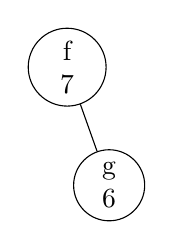
\begin{tikzpicture}[every node/.style = { draw, align = center, shape = circle }]
      \node { f \\ 7 }
      child { node [right = .75mm] { g \\ 6 } };
    \end{tikzpicture}
    \label{subfig:aufg9-i-1-before}
    \caption{Vorher}
  \end{subfigure}
  \quad
  \begin{subfigure}[b]{.4\textwidth}
    \centering
    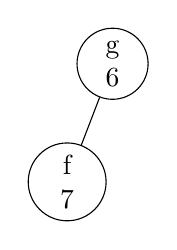
\begin{tikzpicture}[every node/.style = { draw, align = center, shape = circle }]
      \node { g \\ 6 }
      child { node [left = .75mm] { f \\ 7 } };
    \end{tikzpicture}
    \label{subfig:aufg9-i-1-after}
    \caption{Nachher}
  \end{subfigure}
  \label{fig:aufg9-i-1}
  
\end{figure}
Insert $h_{25}$:
\begin{figure}[H]
  \centering
  \begin{subfigure}[b]{.4\textwidth}
    \centering
    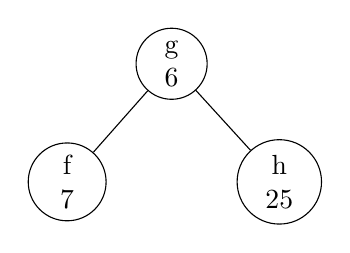
\begin{tikzpicture}[every node/.style = { draw, align = center, shape = circle }]
      \node { g \\ 6 }
      child { node [left = .75mm] { f \\ 7 }}
      child { node [right = .75mm] { h \\ 25 } };
    \end{tikzpicture}
    \label{subfig:aufg9-i-1-before}
    \caption{Keine Rotation notwendig}
  \end{subfigure}
  
\end{figure}
Insert $e_{3}$:
\begin{figure}[H]
  \centering
  \begin{subfigure}[b]{.4\textwidth}
    \centering
    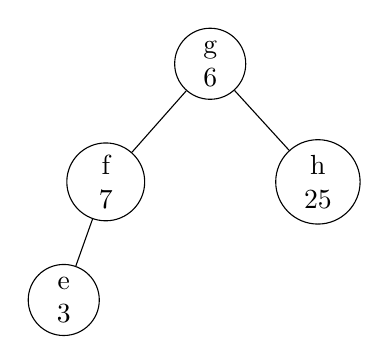
\begin{tikzpicture}[every node/.style = { draw, align = center, shape = circle }]
      \node { g \\ 6 }
      child { node [left = .75mm] { f \\ 7 } 
        child { node [left = .75mm] { e \\ 3 } }
      }
      child { node [right = .75mm] { h \\ 25 } };
    \end{tikzpicture}
    \label{subfig:aufg9-i-1-before}
    \caption{Vorher}
  \end{subfigure}
  \quad
  \begin{subfigure}[b]{.4\textwidth}
    \centering
    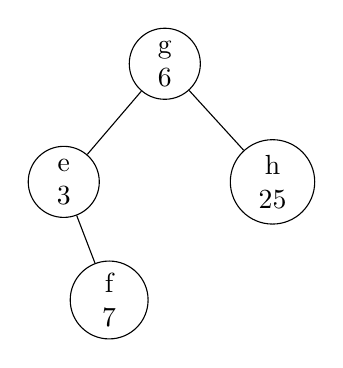
\begin{tikzpicture}[every node/.style = { draw, align = center, shape = circle }]
      \node { g \\ 6 }
      child { node [left = .75mm] { e \\ 3 } 
        child { node [right = .75mm] { f \\ 7 } }
      }
      child { node [right = .75mm] { h \\ 25 } };
    \end{tikzpicture}
    \label{subfig:aufg9-i-1-before}
    \caption{nach: RotiereNachRechts($f_{7}$)}
  \end{subfigure}
  
  \begin{subfigure}[b]{.4\textwidth}
    \centering
    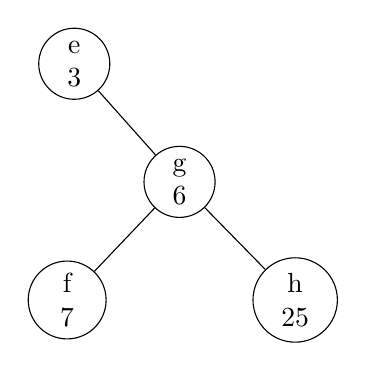
\begin{tikzpicture}[every node/.style = { draw, align = center, shape = circle }]
      \node { e \\ 3 }
      child { node [right = 2.5em] { g \\ 6  } 
        child { node [left = .5em] { f \\ 7 } }
        child { node [right = .5em] { h \\ 25 } } 
      };
    \end{tikzpicture}
    \label{subfig:aufg9-i-1-after}
    \caption{Nachher (nach: RotiereNachRechts($g_{6}$))}
  \end{subfigure}
  \label{fig:aufg9-i-1}
  
\end{figure}
\newpage
Insert $b_{15}$:
\begin{figure}[H]
  \centering
  \begin{subfigure}[b]{.45\textwidth}
    \centering
    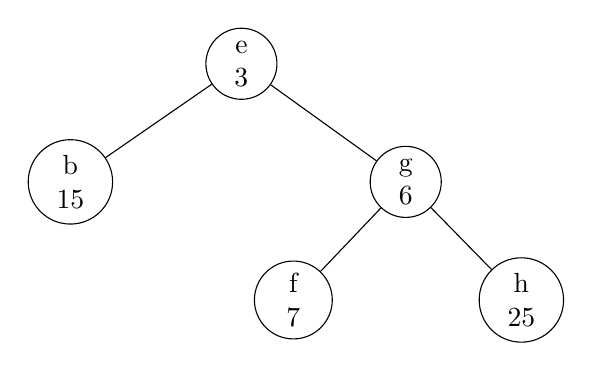
\begin{tikzpicture}[every node/.style = { draw, align = center, shape = circle }]
      \node { e \\ 3 }
      child { node [left = 2.5em] { b \\ 15 }}
      child { node [right = 2.5em] { g \\ 6  } 
        child { node [left = .5em] { f \\ 7 } }
        child { node [right = .5em] { h \\ 25 } } 
      };
    \end{tikzpicture}
    \label{subfig:aufg9-i-1-before}
    \caption{Keine Rotation notwendig}
  \end{subfigure}
 
\end{figure}
Insert $a_{8}$:

\begin{figure}[H]
  \centering
  \begin{subfigure}[b]{.45\textwidth}
    \centering
    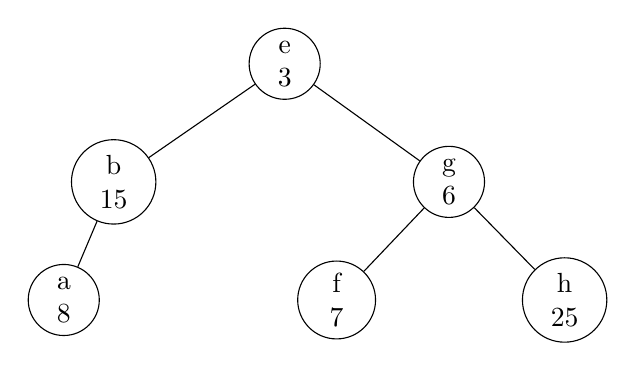
\begin{tikzpicture}[every node/.style = { draw, align = center, shape = circle }]
      \node { e \\ 3 }
      child { node [left = 2.5em] { b \\ 15 }
        child { node [left = .5em] { a \\ 8 } }
      }
      child { node [right = 2.5em] { g \\ 6  } 
        child { node [left = .5em] { f \\ 7 } }
        child { node [right = .5em] { h \\ 25 } } 
      };
    \end{tikzpicture}
    \label{subfig:aufg9-i-1-before}
    \caption{Vorher}
  \end{subfigure}
  \quad
  \begin{subfigure}[b]{.45\textwidth}
    \centering
    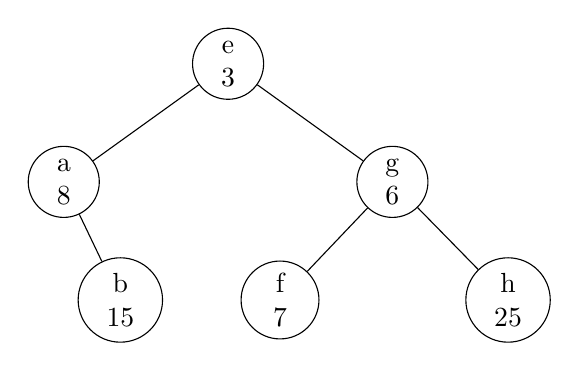
\begin{tikzpicture}[every node/.style = { draw, align = center, shape = circle }]
      \node { e \\ 3 }
      child { node [left = 2.5em] { a \\ 8 }
        child { node [right = .5em] { b \\ 15 } }
      }
      child { node [right = 2.5em] { g \\ 6  } 
        child { node [left = .5em] { f \\ 7 } }
        child { node [right = .5em] { h \\ 25 } } 
      };
    \end{tikzpicture}
    \label{subfig:aufg9-i-1-after}
    \caption{Nachher (nach: RotiereNachRechts($b_{15}$))}
  \end{subfigure}
  \label{fig:aufg9-i-1}

\end{figure}
\newpage
Insert $c_{2}$:
\begin{figure}[H]
  \centering
  \begin{subfigure}[b]{.45\textwidth}
    \centering
    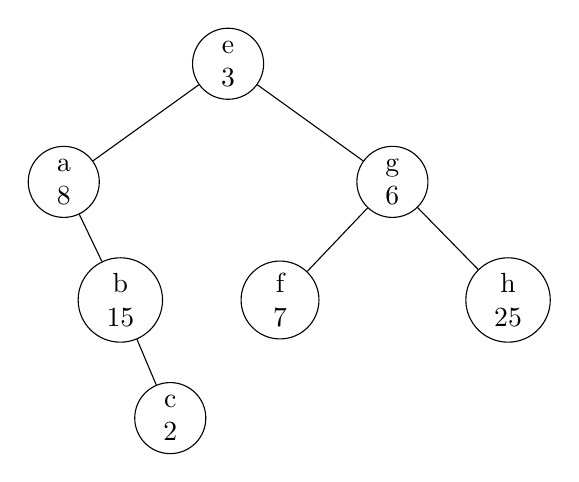
\begin{tikzpicture}[every node/.style = { draw, align = center, shape = circle }]
      \node { e \\ 3 }
      child { node [left = 2.5em] { a \\ 8 }
        child { node [right = .5em] { b \\ 15 } 
          child { node [right = .5em] { c \\ 2 } }
        }
      }
      child { node [right = 2.5em] { g \\ 6  } 
        child { node [left = .5em] { f \\ 7 } }
        child { node [right = .5em] { h \\ 25 } } 
      };
    \end{tikzpicture}
   
    \label{subfig:aufg9-i-1-before}
    \caption{Vorher}
  \end{subfigure}
    \quad
  \begin{subfigure}[b]{.45\textwidth}
    \centering
      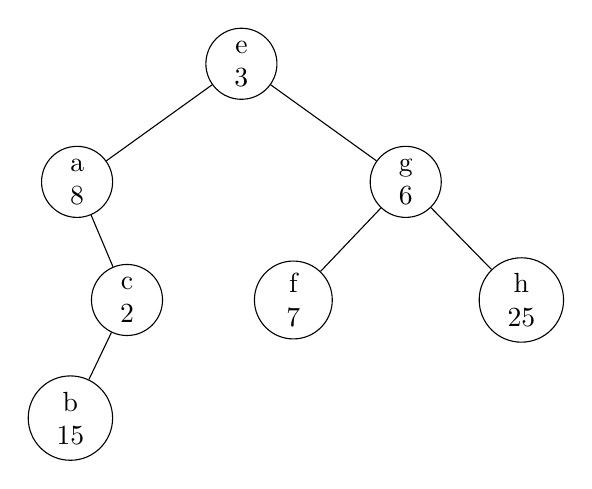
\begin{tikzpicture}[every node/.style = { draw, align = center, shape = circle }]
      \node { e \\ 3 }
      child { node [left = 2.5em] { a \\ 8 }
        child { node [right = .5em] { c \\ 2 } 
          child { node [left = .5em] { b \\ 15} }
        }
      }
      child { node [right = 2.5em] { g \\ 6  } 
        child { node [left = .5em] { f \\ 7 } }
        child { node [right = .5em] { h \\ 25 } } 
      };
    \end{tikzpicture}
    \label{subfig:aufg9-i-1-after}
    \caption{nach: RotiereNachLinks($b_{15}$)}
  \end{subfigure}
  \label{fig:aufg9-i-1}
    \quad
  \begin{subfigure}[b]{.40\textwidth}
    \centering
      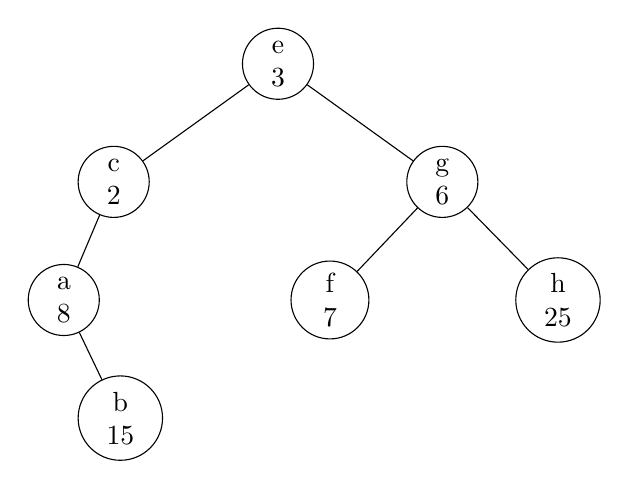
\begin{tikzpicture}[every node/.style = { draw, align = center, shape = circle }]
      \node { e \\ 3 }
      child { node [left = 2.5em] { c \\ 2 }
        child { node [left = .5em] { a \\ 8 } 
          child { node [right = .5em] { b \\ 15} }
        }
      }
      child { node [right = 2.5em] { g \\ 6  } 
        child { node [left = .5em] { f \\ 7 } }
        child { node [right = .5em] { h \\ 25 } } 
      };
    \end{tikzpicture}
    \label{subfig:aufg9-i-1-after}
    \caption{nach: RotiereNachLinks($a_{8}$)}
  \end{subfigure}
  \label{fig:aufg9-i-1}
  \quad
  \begin{subfigure}[b]{.40\textwidth}
    \centering
    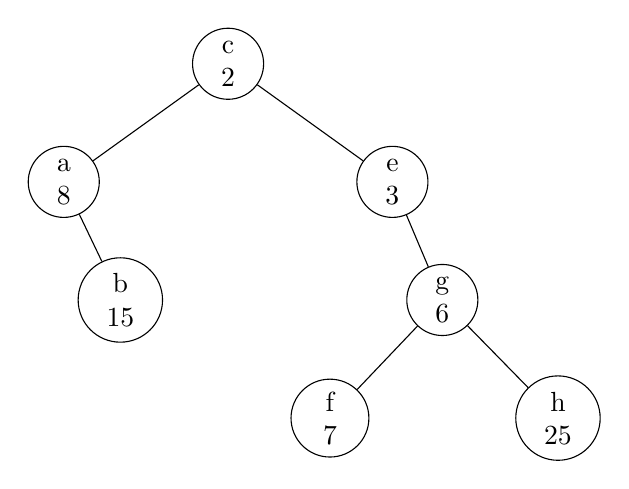
\begin{tikzpicture}[every node/.style = { draw, align = center, shape = circle }]
      \node { c \\ 2 }
      child { node [left = 2.5em] { a \\ 8 }
        child { node [right = .5em] { b \\ 15 } }
      }
      child { node [right = 2.5em] { e \\ 3  } 
        child { node [right = .5em] { g \\ 6 }
        child { node [left = .5em] { f \\ 7 } }
          child { node [right = .5em] { h \\ 25 } }
        }
      };
    \end{tikzpicture}
    \label{subfig:aufg9-i-1-after}
    \caption{Nachher (nach: RotiereNachRechts($e_{3}$))}
  \end{subfigure}
  \label{fig:aufg9-i-1}
  
\end{figure}
\newpage
ii.) Entfernen Sie $e$ aus dem Treap.
\begin{figure}[H]
  \centering
  \begin{subfigure}[b]{.45\textwidth}
    \centering
    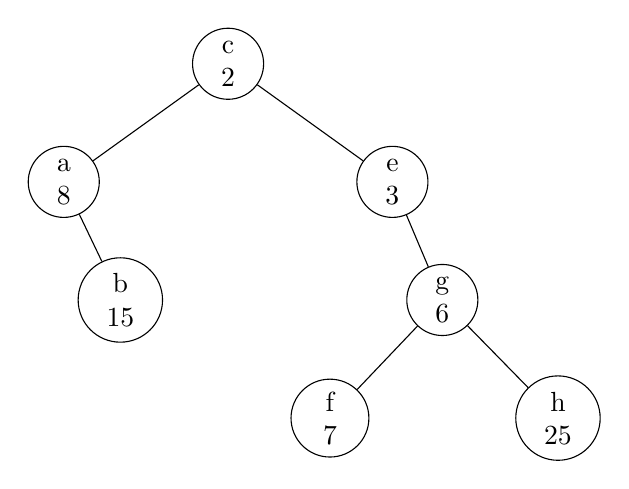
\begin{tikzpicture}[every node/.style = { draw, align = center, shape = circle }]
      \node { c \\ 2 }
      child { node [left = 2.5em] { a \\ 8 }
        child { node [right = .5em] { b \\ 15 } }
      }
      child { node [right = 2.5em] { e \\ 3  } 
        child { node [right = .5em] { g \\ 6 }
        child { node [left = .5em] { f \\ 7 } }
          child { node [right = .5em] { h \\ 25 } }
        }
      };
    \end{tikzpicture}
    \label{subfig:aufg9-i-1-after}
    \caption{Start}
  \end{subfigure}
\end{figure}

\begin{figure}[H]
  \centering
  \begin{subfigure}[b]{.45\textwidth}
    \centering
    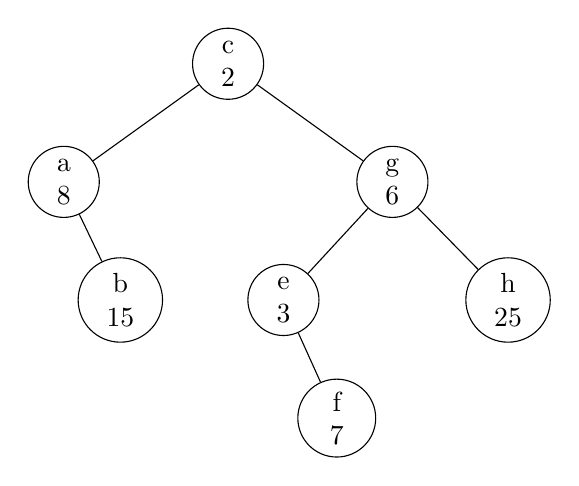
\begin{tikzpicture}[every node/.style = { draw, align = center, shape = circle }]
      \node { c \\ 2 }
      child { node [left = 2.5em] { a \\ 8 }
        child { node [right = .5em] { b \\ 15 } }
      }
      child { node [right = 2.5em] { g \\ 6  } 
        child { node [left = .5em] { e \\ 3 } 
        	child { node [right = .5em] { f \\ 7 }}} 
        child { node [right = .5em] { h \\ 25 } } 
      };
      
    \end{tikzpicture}
    \label{subfig:aufg9-i-1-after}
    \caption{nach: $g_{6}$ is rechtes Kind von $e_{3}$ $\implies$ RotiereNachLinks($e_{3}$)}
  \end{subfigure}
  \quad
  \begin{subfigure}[b]{.45\textwidth}
    \centering
    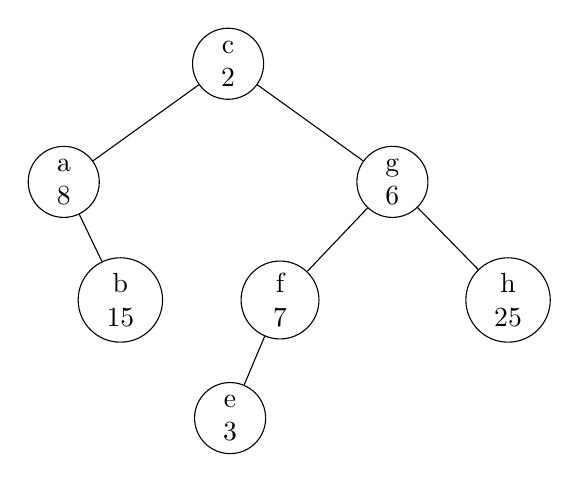
\begin{tikzpicture}[every node/.style = { draw, align = center, shape = circle }]
      \node { c \\ 2 }
      child { node [left = 2.5em] { a \\ 8 }
        child { node [right = .5em] { b \\ 15 } }
      }
      child { node [right = 2.5em] { g \\ 6  } 
        child { node [left = .5em] { f \\ 7 } 
        	child { node [left = .5em] { e \\ 3 }}} 
        child { node [right = .5em] { h \\ 25 } } 
      };
      
    \end{tikzpicture}
    \label{subfig:aufg9-i-1-after}
    \caption{nach: $f_{7}$ is rechtes Kind von $e_{3}$ $\implies$ RotiereNachLinks($e_{3}$)}
  \end{subfigure}
\end{figure}

\begin{figure}[H]
  \centering
\begin{subfigure}[b]{.45\textwidth}
    \centering
    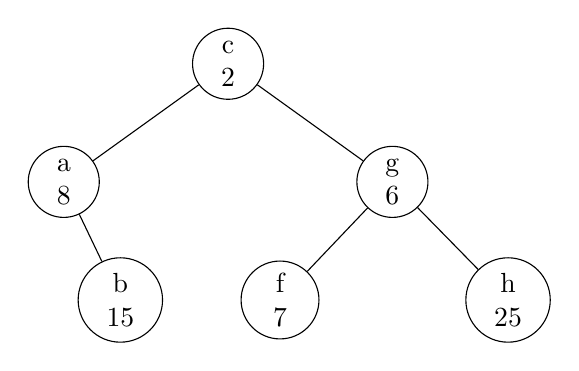
\begin{tikzpicture}[every node/.style = { draw, align = center, shape = circle }]
      \node { c \\ 2 }
      child { node [left = 2.5em] { a \\ 8 }
        child { node [right = .5em] { b \\ 15 } }
      }
      child { node [right = 2.5em] { g \\ 6  } 
        child { node [left = .5em] { f \\ 7 } }       	 
        child { node [right = .5em] { h \\ 25 } } 
      };
      
    \end{tikzpicture}
    \label{subfig:aufg9-i-1-after}
    \caption{Ende}
  \end{subfigure}
\end{figure}
\newpage
iii.) F{\"u}gen Sie die Schl{\"u}ssel $i_{22}$, $j_{19}$, $k_{13}$ in einen anderen (anfangs
    leeren) Treap ein. Vereinigen Sie anschlie{\ss}end die zwei Treaps.

Insert $j_{19}$:
\begin{figure}[H]
  \centering
  \begin{subfigure}[b]{.4\textwidth}
    \centering
    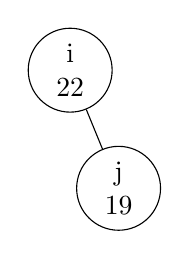
\begin{tikzpicture}[every node/.style = { draw, align = center, shape = circle }]
      \node { i \\ 22 }
      child { node [right = .75mm] { j \\ 19 } };
    \end{tikzpicture}
    \label{subfig:aufg9-i-1-before}
    \caption{Vorher}
  \end{subfigure}
  \quad
  \begin{subfigure}[b]{.4\textwidth}
    \centering
    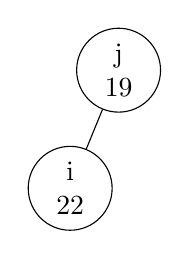
\begin{tikzpicture}[every node/.style = { draw, align = center, shape = circle }]
      \node { j \\ 19 }
      child { node [left = .75mm] { i \\ 22 } };
    \end{tikzpicture}
    \label{subfig:aufg9-i-1-after}
    \caption{Nachher (nach: RotiereNachLinks($i_{22}$))}
  \end{subfigure}
  \label{fig:aufg9-i-1} 
\end{figure}
Insert $k_{13}$:
\begin{figure}[H]
 
  \begin{subfigure}[b]{.4\textwidth}
    \centering
    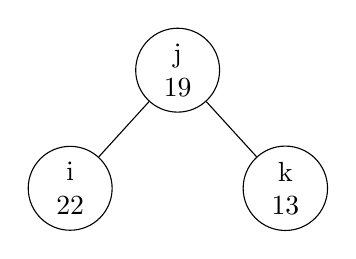
\begin{tikzpicture}[every node/.style = { draw, align = center, shape = circle }]
      \node { j \\ 19 }
      child { node [left = .75mm] { i \\ 22 } }
      child { node [right = .75mm] { k \\ 13 } };
    \end{tikzpicture}
    \label{subfig:aufg9-i-1-after}
    \caption{Vorher}
  \end{subfigure}
  \quad
  \begin{subfigure}[b]{.4\textwidth}
    \centering
    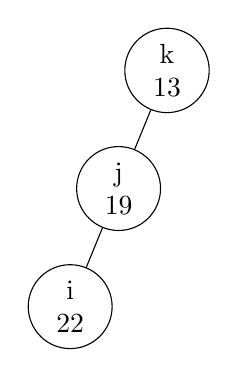
\begin{tikzpicture}[every node/.style = { draw, align = center, shape = circle }]
      \node { k \\ 13 }
      child { node [left = .75mm] { j \\ 19 } 
      child { node [left = .75mm] { i \\ 22 } }};
    \end{tikzpicture}
    \label{subfig:aufg9-i-1-after}
    \caption{Nachher (nach: RotiereNachLinks($j_{19}$))}
  \end{subfigure}
  \label{fig:aufg9-i-1} 
\end{figure}
\newpage
Vereinige($T_1$,$T_2$):
\begin{figure}[H]
 
  \begin{subfigure}[b]{.4\textwidth}
    \centering
    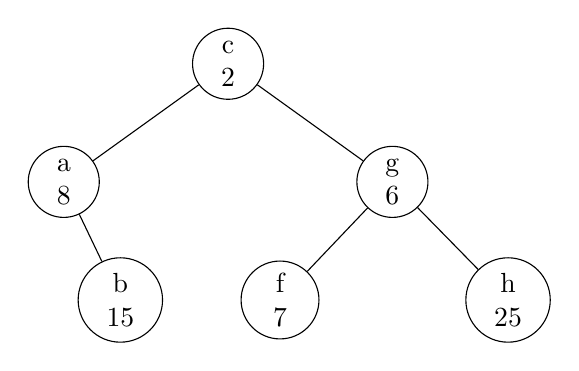
\begin{tikzpicture}[every node/.style = { draw, align = center, shape = circle }]
      \node { c \\ 2 }
      child { node [left = 2.5em] { a \\ 8 }
        child { node [right = .5em] { b \\ 15 } }
      }
      child { node [right = 2.5em] { g \\ 6  } 
        child { node [left = .5em] { f \\ 7 } }       	 
        child { node [right = .5em] { h \\ 25 } } 
      };
      
    \end{tikzpicture}
    \label{subfig:aufg9-i-1-after}
    \caption{$T_1$}
  \end{subfigure}
  \quad
  \begin{subfigure}[b]{.4\textwidth}
    \centering
    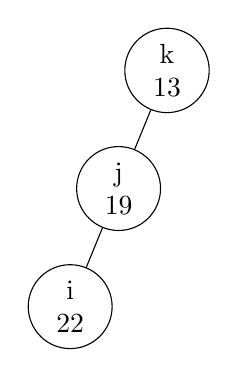
\begin{tikzpicture}[every node/.style = { draw, align = center, shape = circle }]
      \node { k \\ 13 }
      child { node [left = .75mm] { j \\ 19 } 
      child { node [left = .75mm] { i \\ 22 } }};
    \end{tikzpicture}
    \label{subfig:aufg9-i-1-after}
    \caption{$T_2$}
  \end{subfigure}
  \label{fig:aufg9-i-1} 
\end{figure}
Sei $\dot{k}$ ein Schlüssel mit key($x_1$) $<$ $\dot{k}$ $<$ key($x_2$) für alle $x_1 \in T_1$ und $x_2 \in T_2$. Ein echter Buchstabe kann hier nicht verwendet werden, da ein solcher im deutschen Alphabet (natürliche Ordnung) nicht existiert. Es gilt also: $a < b < c < ... < \dot{k} < i < j < k < ... < z$.

\begin{figure}[H]
     \centering
  \begin{subfigure}[b]{.4\textwidth}
    \centering
    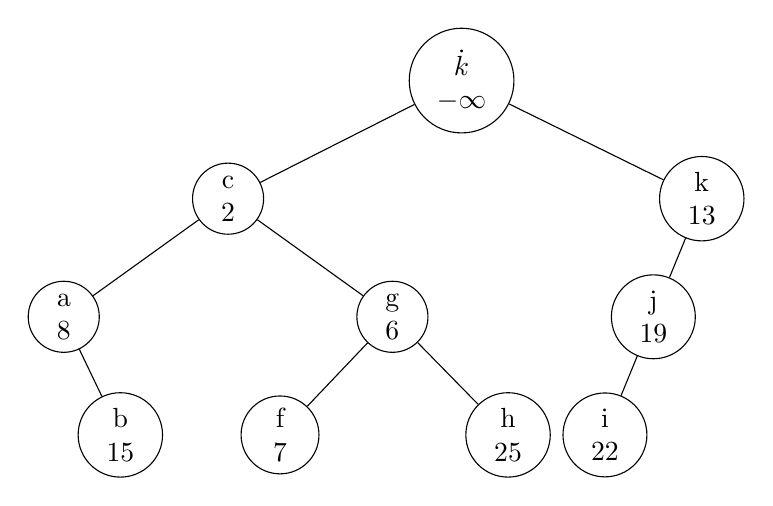
\begin{tikzpicture}[every node/.style = { draw, align = center, shape = circle }]
    	 \node { $\dot{k}$ \\ $-\infty$ }
      child { node [left = 5em] { c \\ 2 }
      child { node [left = 2.5em] { a \\ 8 }
        child { node [right = .5em] { b \\ 15 } }
      }
      child { node [right = 2.5em] { g \\ 6  } 
        child { node [left = .5em] { f \\ 7 } }       	 
        child { node [right = .5em] { h \\ 25 } } 
      }}
      child { node [right = 5em] { k \\ 13 }
      child { node [left = .75mm] { j \\ 19 } 
      child { node [left = .75mm] { i \\ 22 } }}};
      
    \end{tikzpicture}
    \label{subfig:aufg9-i-1-after}
    \caption{Neuer Knoten mit Schlüssel $\dot{k}$ als Wurzel.}
  \end{subfigure} 
  \label{fig:aufg9-i-1} 
\end{figure}
\newpage

Entferne Wurzel aus Treap:
\begin{figure}[H]
   \scalebox{.7}{
  \begin{subfigure}[b]{.7\textwidth}
    \centering
    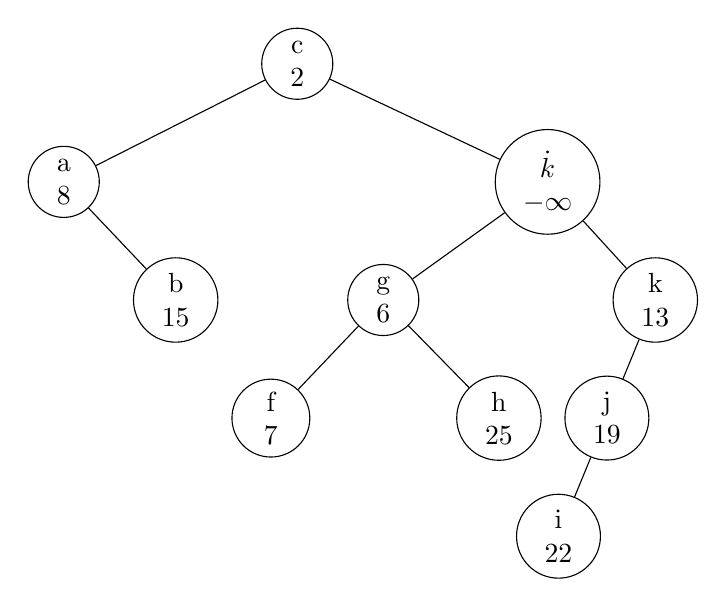
\begin{tikzpicture}[every node/.style = { draw, align = center, shape = circle }]
    	 \node { c \\ 2 }
      child { node [left = 5em] { a \\ 8 }
      child { node [right = 2.5em] { b \\ 15 } }
     }
      child { node [right = 5em] { $\dot{k}$ \\ $-\infty$ }
       child { node [left = 2.5em] { g \\ 6  } 
        child { node [left = .5em] { f \\ 7 } }       	 
        child { node [right = .5em] { h \\ 25 } } 
      }
      child { node [right= .75mm] { k \\ 13 } 
      child { node [left= .75mm] { j \\ 19 } 
      child { node [left = .75mm] { i \\ 22 } }}}};
      
    \end{tikzpicture}
    \label{subfig:aufg9-i-1-after}
    \caption{nach: $c_{2}$ is linkes Kind von $\dot{k}_{-\infty}$ $\implies$ 			RotiereNachRechts($\dot{k}_{-\infty}$)}
  \end{subfigure} 
  }
  \quad
	\scalebox{.7}{
  \begin{subfigure}[b]{.7\textwidth}
    \centering
    \begin{tikzpicture}[every node/.style = { draw, align = center, shape = circle }]
    	 \node { c \\ 2 }
      child { node [left = 5em] { a \\ 8 }
      child { node [right = 2.5em] { b \\ 15 } }
     }
      child { node [right = 5em] { g\\ 6 }
       child { node [left = 2.5em] { f \\ 7  } 
      }
      child { node [right = 5em] { $\dot{k}$ \\ $-\infty$ }
      child { node [left= .75mm] { h \\ 25 }}
      child { node [right= .75mm] { k \\ 13 } 
      child { node [left= .75mm] { j \\ 19 } 
      child { node [left = .75mm] { i \\ 22 } }}}}};
      
    \end{tikzpicture}
    \label{subfig:aufg9-i-1-after}
    \caption{nach: $g_{6}$ is linkes Kind von $\dot{k}_{-\infty}$ $\implies$ 			RotiereNachRechts($\dot{k}_{-\infty}$)}
  \end{subfigure} 
  }
  \quad
  \scalebox{.7}{
  \begin{subfigure}[b]{.7\textwidth}
    \centering
    \begin{tikzpicture}[every node/.style = { draw, align = center, shape = circle }]
    	 \node { c \\ 2 }
      child { node [left = 5em] { a \\ 8 }
      child { node [right = 2.5em] { b \\ 15 } }
     }
      child { node [right = 5em] { g\\ 6 }
       child { node [left = 2.5em] { f \\ 7  } 
      }
      child { node [right = 5em] {k \\ 13  }
      child { node [left= .75mm] { $\dot{k}$ \\ $-\infty$}
      child { node [left= .75mm] { h \\ 25 }}
      child { node [right= .75mm] { j \\ 19 } 
      child { node [left = .75mm] { i \\ 22 } }}}}};
      
    \end{tikzpicture}
    \label{subfig:aufg9-i-1-after}
    \caption{nach: $k_{13}$ is rechtes Kind von $\dot{k}_{-\infty}$ $\implies$ 			RotiereNachLinks($\dot{k}_{-\infty}$)}
  \end{subfigure} 
  }
  \quad
  \scalebox{.7}{
  \begin{subfigure}[b]{.7\textwidth}
    \centering
    \begin{tikzpicture}[every node/.style = { draw, align = center, shape = circle }]
    	 \node { c \\ 2 }
      child { node [left = 5em] { a \\ 8 }
      child { node [right = 2.5em] { b \\ 15 } }
     }
      child { node [right = 5em] { g\\ 6 }
       child { node [left = 2.5em] { f \\ 7  } 
      }
      child { node [right = 5em] {k \\ 13  }
      child { node [left= .75mm] { j \\ 19}
      child { node [left= .75mm] { $\dot{k}$ \\ $-\infty$}
      child { node [left= .75mm] { h \\ 25 } }
      child { node [right = .75mm] { i \\ 22 } }}}}};
      
    \end{tikzpicture}
    \label{subfig:aufg9-i-1-after}
    \caption{nach: $j_{19}$ is rechtes Kind von $\dot{k}_{-\infty}$ $\implies$ 			RotiereNachLinks($\dot{k}_{-\infty}$)}
  \end{subfigure} 
  }
 	\quad
 	\scalebox{.7}{
  \begin{subfigure}[b]{.7\textwidth}
    \centering
    \begin{tikzpicture}[every node/.style = { draw, align = center, shape = circle }]
    	 \node { c \\ 2 }
      child { node [left = 5em] { a \\ 8 }
      child { node [right = 2.5em] { b \\ 15 } }
     }
      child { node [right = 5em] { g\\ 6 }
       child { node [left = 2.5em] { f \\ 7  } 
      }
      child { node [right = 5em] {k \\ 13  }
      child { node [left= .75mm] { j \\ 19}
      child { node [left= .75mm] { i \\22}
      child { node [left= .75mm] { $\dot{k}_{-\infty}$ }
      child { node [left= .75mm] {h \\ 25}  }
      }}}}};
      
    \end{tikzpicture}
    \label{subfig:aufg9-i-1-after}
    \caption{nach: $i_{22}$ is rechtes Kind von $\dot{k}_{-\infty}$ $\implies$ 			RotiereNachLinks($\dot{k}_{-\infty}$)}
  \end{subfigure} 
}  
\quad
\scalebox{.7}{
  \begin{subfigure}[b]{.7\textwidth}
    \centering
    \begin{tikzpicture}[every node/.style = { draw, align = center, shape = circle }]
    	 \node { c \\ 2 }
      child { node [left = 5em] { a \\ 8 }
      child { node [right = 2.5em] { b \\ 15 } }
     }
      child { node [right = 5em] { g\\ 6 }
       child { node [left = 2.5em] { f \\ 7  } 
      }
      child { node [right = 5em] {k \\ 13  }
      child { node [left= .75mm] { j \\ 19}
      child { node [left= .75mm] { i \\22}
      child { node [left= .75mm] { h \\ 25 }
      child { node [left= .75mm] {$\dot{k}_{-\infty}$}  }
      }}}}};
      
    \end{tikzpicture}
    \label{subfig:aufg9-i-1-after}
    \caption{nach: $h_{25}$ ist linkes Kind von $\dot{k}_{-\infty}$ $\implies$ 			RotiereNachRechts($\dot{k}_{-\infty}$)\\
    Der Hilfsknoten $\dot{k}_{-\infty}$ ist jetzt ein Blatt und kann einfach entfernt werden.}
  \end{subfigure} 
  }
  \label{fig:aufg9-i-1} 
\end{figure}



\newpage
iv.)F{\"u}hren Sie $Spalte \left( T, d, T_1, T_2 \right)$ durch, wobei $T$
    der Treap aus dem vorigen Punkt ist.

Füge Knoten $d_{-\infty}$ in T ein:
   \begin{figure}[H]
   \scalebox{.7}{
  \begin{subfigure}[b]{.7\textwidth}
    \centering
    \begin{tikzpicture}[every node/.style = { draw, align = center, shape = circle }]
    	 \node { c \\ 2 }
      child { node [left = 5em] { a \\ 8 }
      child { node [right = 2.5em] { b \\ 15 } }
     }
      child { node [right = 5em] { g\\ 6 }
       child { node [left = 2.5em] { f \\ 7  } 
       child { node [left = 2.5em] { d \\ $-\infty$  }}
      }
      child { node [right = 5em] {k \\ 13  }
      child { node [left= .75mm] { j \\ 19}
      child { node [left= .75mm] { i \\22}
      child { node [left= .75mm] { h \\ 25 }     
      }}}}};
      
    \end{tikzpicture}
    \label{subfig:aufg9-i-1-after}
    \caption{Vorher}
  \end{subfigure} 
  }
  \quad
 \scalebox{.7}{
  \begin{subfigure}[b]{.7\textwidth}
   
    \begin{tikzpicture}[every node/.style = { draw, align = center, shape = circle }]
    	 \node { c \\ 2 }
      child { node [left = 5em] { a \\ 8 }
      child { node [right = 2.5em] { b \\ 15 } }
     }
      child { node [right = 5em] { g\\ 6 }
       child { node [left = 2.5em] { d \\ $-\infty$  } 
       child { node [right = 2.5em] { f \\ 7  }}
      }
      child { node [right = 5em] {k \\ 13  }
      child { node [left= .75mm] { j \\ 19}
      child { node [left= .75mm] { i \\22}
      child { node [left= .75mm] { h \\ 25 }     
      }}}}};
      
    \end{tikzpicture}
    \label{subfig:aufg9-i-1-after}
    \caption{nach: $d_{-\infty}$ ist linkes Kind von $f_7$ $\implies$ 			RotiereNachRechts($f_7$)}
  \end{subfigure} 
  }

	\quad
    
   \scalebox{.7}{
  \begin{subfigure}[b]{.7\textwidth}

      \begin{tikzpicture}[every node/.style = { draw, align = center, shape = circle }]
    	 \node { c \\ 2 }
      child { node [left = 2.5em] { a \\ 8 }
      child { node [right = 2.5em] { b \\ 15 } }
     }
      child { node [right = 2.5em] { d\\ $-\infty$ }
      child {node [right = 5em] { g\\ 6 }
      child { node [left= .75mm] { f \\ 7}}
      child { node [right = .75em] {k \\ 13  }
      child { node [left= .75mm] { j \\ 19}
      child { node [left= .75mm] { i \\22}
      child { node [left= .75mm] { h \\ 25 }     
      }}}}}};
      
    \end{tikzpicture}
    \label{subfig:aufg9-i-1-after}
    \caption{nach: $d_{-\infty}$ ist linkes Kind von $g_6$ $\implies$ 			RotiereNachRechts($g_6$)}
  \end{subfigure} 
	}
\quad
 \scalebox{.7}{
  \begin{subfigure}[b]{.7\textwidth}
   
    
    \begin{tikzpicture}[every node/.style = { draw, align = center, shape = circle }]
    \node { d\\ $-\infty$  }
      child { node [left = 2.5em] { c \\ 2 }
      child { node [left = 2.5em] { a \\ 8 }
      child { node [right = 2.5em] { b \\ 15 } }}}
      child {node [right = 5em] { g\\ 6 }
      child { node [left= .75mm] { f \\ 7}}
      child { node [right = .75em] {k \\ 13  }
      child { node [left= .75mm] { j \\ 19}
      child { node [left= .75mm] { i \\22}
      child { node [left= .75mm] { h \\ 25 }     
      }}}}};
      
    \end{tikzpicture}
    \label{subfig:aufg9-i-1-after}
    \caption{nach: $d_{-\infty}$ ist rechtes Kind von $c_2$ $\implies$ 			RotiereNachLinks($c_2$)}
  \end{subfigure} 
	}
\quad

 \scalebox{.7}{
  \begin{subfigure}[b]{.7\textwidth}
   
    
    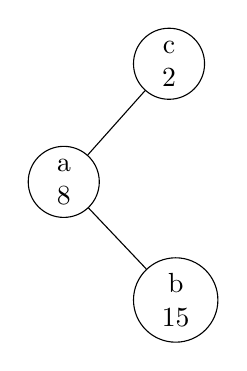
\begin{tikzpicture}[every node/.style = { draw, align = center, shape = circle }]
    \node { c \\ 2 }
      child { node [left = 2.5em] { a \\ 8 }
      child { node [right = 2.5em] { b \\ 15 } }};
      
      
    \end{tikzpicture}
    \label{subfig:aufg9-i-1-after}
    \caption{$T_1$}
  \end{subfigure} 
	}
	\quad
 \scalebox{.7}{
  \begin{subfigure}[b]{.7\textwidth}
   
    
    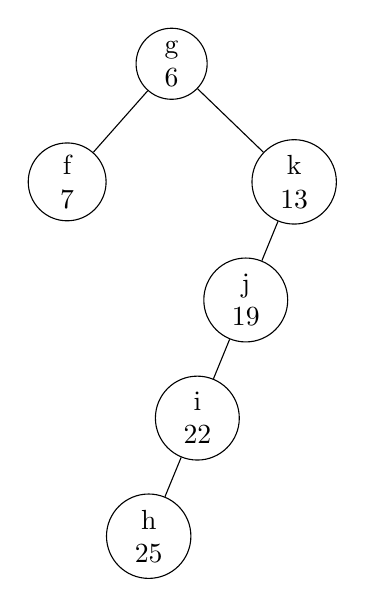
\begin{tikzpicture}[every node/.style = { draw, align = center, shape = circle }]
    \node { g\\ 6  }            
      child { node [left= .75mm] { f \\ 7}}
      child { node [right = .75em] {k \\ 13  }
      child { node [left= .75mm] { j \\ 19}
      child { node [left= .75mm] { i \\22}
      child { node [left= .75mm] { h \\ 25 }     
      }}}};
      
    \end{tikzpicture}
    \label{subfig:aufg9-i-1-after}
    \caption{$T_2$}
  \end{subfigure} 
	}
  \label{fig:aufg9-i-1} 
\end{figure}
\newpage
{\bfseries Aufgabe 12}%

Der {\it linke Rand} in einem bin{\"a}ren Suchbaum $T$ ist der Pfad von der Wurzel
zum Knoten mit dem kleinsten Schl{\"u}ssel. Der {\it rechte Rand} in einem
bin{\"a}ren Suchbaum $T$ ist der Pfad von der Wurzel zum Knoten mit dem
gr{\"o}{\ss}ten Schl{\"u}ssel. Betrachten Sie einen Treap $T$ direkt nach dem
Einf{\"u}gen eines Objektes $x$. Sei $C$ die L{\"a}nge des rechten Randes des
linken Unterbaums des Knotens mit dem Element $x$ und sei $D$ die L{\"a}nge des
linken Randes des rechten Unterbaums des Knotens mit dem Element $x$. Zeigen Sie,
dass die Anzahl der Rotationen, die w{\"a}hrend des Einf{\"u}gens von $x$
durchgef{\"u}hrt wurden, $C + D$ ist.

\medskip%

Linker Rand eines bin{\"a}ren Suchbaums: von der Wurzel zum linkesten Kind, d.h.
verfolge ausgehend von der Wurzel immer die Kante zum linken Kind.
\newline
Rechter Rand eines bin{\"a}ren Suchbaums: analog (verfolge immer die Kante zum
rechten Kind).

$C$ \ldots L{\"a}nge des rechten Randes des linken Unterbaums des Knotens mit dem
Element $x$.
\newline
$D$ \ldots L{\"a}nge des linken Randes des rechten Unterbaums des Knotens mit dem
Element $x$.
\newline
$R$ \ldots \# der Rotationen, die w{\"a}hrend des Einf{\"u}gens von $x$
durchgef{\"u}hrt wurden.


Zu zeigen: $C + D = R$

\begin{proof}
Ausgehend von der Annahme, dass $C + D = R$ vor der ersten Rotation gilt,
zeigen wir nun, dass $C + D = R$ auch nach der darauffolgenden Rotation gilt.

{\bfseries I.A.:} $C + D = 0$ gilt trivialerweise, da $C = D = 0$.

{\bfseries I.B.:} $C + D = R$ gilt f{\"u}r $N$ Rotation.

{\bfseries I.S.:}
Seien $C$, $D$, $C_{NR}$ und $D_{NR}$ wie folgt:

$C$ \ldots L{\"a}nge des rechten Randes des linken Unterbaums des Knotens mit
dem Element $x$ \emph{vor der Rotation}.
\newline
$D$ \ldots L{\"a}nge des linken Randes des rechten Unterbaums des Knotens mit
dem Element $x$ \emph{vor der Rotation}.
\newline
$C_{NR}$ \ldots L{\"a}nge des rechten Randes des linken Unterbaums des Knotens
mit dem Element $x$ \emph{nach der Rotation}.
\newline
$D_{NR}$ \ldots L{\"a}nge des linken Randes des rechten Unterbaums des Knotens
mit dem Element $x$ \emph{nach der Rotation}.

Es gibt nun zwei F{\"a}lle zu unterscheiden.

\underline{Fall 1: Linksrotation bzgl. Knoten $x$}

Vor der Rotation hat der linke Rand des rechten Unterbaums von $x$ die L{\"a}nge
$D$. Analog hat der rechte Rand des linken Unterbaums von $x$ die L{\"a}nge $C$.

Bei einer Linksrotation passiert Folgendes. Sei $y$ der Elternknoten von $x$ vor
der Linksrotation.
{\parskip0pt\begin{itemize}
  \item $x$ wird auf die Position von $y$ geschoben und $y$ wird linkes Kind von
    $x$.
  \item Der linke Unterbaum von $x$ wird zum rechten Unterbaum von $y$.
  \item Der rechte Unterbaum von $x$ bleibt dessen rechter Unterbaum.
  \item Der linke Unterbaum von $y$ bleibt dessen linker Unterbaum.
\end{itemize}}

\begin{figure}[H]
  \centering
  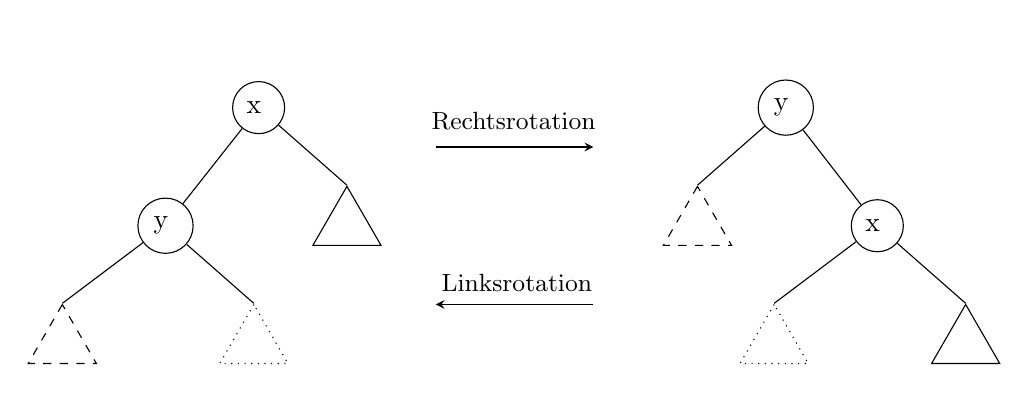
\begin{tikzpicture}[every node/.style = { draw, align = center, shape = circle }, level distance = 1.5cm]
    \node (x1) { x }
    child { node [left = .75mm] { y }
      child[child anchor = north] { node [left = .75em, regular polygon, dashed, regular polygon sides = 3, minimum height = 1cm] { } }
      child[child anchor = north] { node [right = .75mm, regular polygon, dotted, regular polygon sides = 3, minimum height = 1cm] { } }
    }
    child[child anchor = north] { node [right = .75mm, regular polygon, regular polygon sides = 3, minimum height = 1cm] { } };

    \node[right = 6 of x1] { y }
    child[child anchor = north] { node [left = .75mm, regular polygon, dashed, regular polygon sides = 3, minimum height = 1cm] { } }
    child { node [right = .75mm] { x }
      child[child anchor = north] { node [left = .75em, regular polygon, dotted, regular polygon sides = 3, minimum height = 1cm] { } }
      child[child anchor = north] { node [right = .75mm, regular polygon, regular polygon sides = 3, minimum height = 1cm] { } }
    };

    \draw[->, >=stealth] (x1) ++(2.25, -0.5) node[above right = -0.5 and 0.15, draw = none] {\small Rechtsrotation} -- ++(2, 0);
    \draw[<-, >=stealth] (x1) ++(2.25, -2.5) node[above right = -0.5 and 0.25, draw = none] {\small Linksrotation} -- ++(2, 0);
  \end{tikzpicture}
  \label{fig:aufg12-left-rot-x}
  \caption{Links- und Rechtsrotation bzgl. $x$}
\end{figure}

Durch die "Nach-Unten-Verschiebung" des linken Unterbaums von $x$ um eine Ebene,
wird der rechte Rand des linken Unterbaums des Knotens mit dem Element $x$
ebenfalls um 1 l{\"a}nger, d.h. $C_{NR} = C + 1$. Die L{\"a}nge des linken Randes
des rechten Unterbaums des Knotens mit dem Element $x$ bleibt hingegen
unver{\"a}ndert, d.h. $D_{NR} = D$.

F{\"u}r diesen Fall gilt also f{\"u}r $N$ Rotationen, dass $C$
$N$-mal um 1 l{\"a}nger wird, d.h.
$C_{NR} = C + \sum^{N - 1}_{i = 1} 1 = C + N = N$. $D_{NR}$ bleibt hingegen
immer gleich bleibt, d.h. $D_{NR} = D = 0$.

Daraus folgt: $C_{NR} + D_{NR} = N = N$ f{\"u}r $N$ Rotationen. \hfill$\Box$

\underline{Fall 2: Rechtsrotation bzgl. Knoten $x$}

Die selbe Argumentation kann f{\"u}r die Rechtsrotation verwendet werden. Der
einzige Unterschied liegt in der Ver{\"a}nderung des Baumes. Bei einer
Rechtsrotation gilt Folgendes. Sei $y$ das linke Kind von $x$ vor der
Rechtsrotation.
{\parskip0pt\begin{itemize}
  \item $y$ wird der neue Elternknoten von $x$.
  \item Der linke Unterbaum von $y$ bleibt dessen linker Unterbaum.
  \item Der rechte Unterbaum von $y$ wird linker Unterbaum von $x$.
  \item $x$ wird das rechte Kind von $y$.
\end{itemize}}

In diesem Fall wir der Pfad $D$ um 1 l{\"a}nger und $C$ bleibt unver{\"a}ndert,
d.h. $D_{NR} = D + 1$ und $C_{NR} = C$.

Analog zu Fall 1 ergibt sich daraus f{\"u}r $N$ Rotationen:
$C_{NR} + D_{NR} = N = N$. \hfill$\Box$

Das hei{\ss}t, dass $C + D = R$ auch f{\"u}r die Kombination von Links- und
Rechtsrotationen gilt, da nur entweder $D$ oder $C$ um 1 l{\"a}nger werden.
\end{proof}

{\bfseries Aufgabe 13}%

Sei $U = \left\{ 0, \ldots, N - 1 \right\}$, wobei $N$ eine Primzahl ist und sei
$m = 4$. Seien $a_i = 40i$ und $b_i = 60i$. Wir definieren folgende Klasse von
Hashfunktionen:
\begin{equation}
  H = \left\{ h_i \left( k \right) = \left( \left( a_ik + b_i \right)\text{ mod }N - 1 \right)\text{ mod }m \right\}
  \text{ f{\"u}r } i \in \left\{ 1, \ldots, N \left( N - 1 \right) \right\}
\end{equation}
Ist $H$ universell? Warum? Falls $H$ nicht universell ist, so modifizieren Sie
$h_i$, $a_i$ und $b_i$, sodass Sie eine universelle Klasse erhalten.

\medskip%

$H$ ist nicht universell.

\begin{proof}
Da $N$ prim ist, wissen wir, dass (1) $(N - 1)$ keine Primzahl ist (au{\ss}er
$N = 3$) und (2) $(N - 1)$ eine gerade Zahl ist (da alle Primzahlen au{\ss}er
$2$ ungerade sind).

Weiters wissen wir, dass $a_i = 40i$ und $b_i=60i$ beides gerade Zahlen sind,
da eine Multiplikation mit einer geraden Zahl immer eine gerade Zahl ergibt.

%\begin{equation}
%  a_i = 40i = 2c\qquad\text{und}\qquad b_i = 60i = 2d
%\end{equation}

Dies hat zur Folge, dass
$H = \left\{ h_i \left( k \right) = \left( 40ik + 60i \right)\text{ mod } N - 1 \text{ mod } 4 \right\}$
immer eine gerade Zahl ergibt (gerade Zahl mod gerader Zahl ergibt immer gerade
Zahl). Dadurch wird nur der halbe Bereich von $m$ ausgenutzt (n{\"a}mlich nur
jede zweite - gerade - Zahl), d.h. nur $\frac{m}{2}$.

Damit $H$ universell ist, muss nun Folgendes f{\"u}r $\left( x, y \right)$ mit
$x \neq y$ erf{\"u}llt sein:
\begin{equation}
  \frac{|\left\{ h \in H: h\left( x \right) = h\left( y \right) \right\}|}{|H|} \leq \frac{1}{m}
  \Longleftrightarrow
  |\left\{ h \in H: h\left( x \right) = h\left( y \right) \right\}| \leq \frac{|H|}{m}
\end{equation}

Da $i \in \left\{ 1, \ldots, N \left( N - 1 \right) \right\}$, ist
$|H| = N \left( N - 1 \right)$. Weiters ist $m = 4$. Da nur jede zweite -
gerade - Zahl aus dem Wertebereich von $m$ genutzt wird, ist
$|\left\{ h \in H: h\left( x \right) = h\left( y \right) \right\}| = \frac{|H|}{2} = \frac{N \left( N - 1 \right)}{2}$.
Eingesetzt in (2) ergibt sich dadurch
\begin{equation}
  \frac{N \left( N - 1 \right)}{2} \leq \frac{N \left( N - 1 \right)}{4}
  \Longleftrightarrow
  \frac{1}{2} \leq \frac{1}{4}
\end{equation}

(3) ist nicht erf{\"u}llt $\Rightarrow$ $H$ ist nicht universell.
\end{proof}

Damit $H$ universell ist, halten wir uns nun an den Satz von Folie 20:
\begin{equation}
  H = \left\{ h_{a, b} \left( x \right) | 1 \leq a < N \land 0 \leq b < N \right\}
\end{equation}
ist eine universelle Klasse von Hash-Funktionen.

Das hei{\ss}t, wir m{\"u}ssen $a_i$, $b_i$ und $h_i$ so anpassen, dass Folgendes
gilt:
\begin{equation}
  a_i \in \left\{ 1, \ldots, N - 1 \right\},
  b_i \in \left\{ 0, \ldots, N - 1 \right\},
  h_i \left( x \right) = \left( \left( a_ik + b_i \right)\text{ mod } N \right)\text{ mod } m
\end{equation}

Es wurde in der Vorlesung bewiesen, dass diese Klasse von Hash-Funktionen
universell ist.

\clearpage

\begin{equation}
  a_i = f \left( i, N \right),
  f \left( i, N \right) \in \left\{ 1, \ldots, N - 1 \right\}\text{ f{\"u}r }
  i \in \left\{ 1, \ldots, N \left( N - 1 \right) \right\}
\end{equation}

\begin{equation}
  b_i = g \left( i, N \right),
  g \left( i, N \right) \in \left\{ 0, \ldots, N - 1 \right\}\text{ f{\"u}r }
  i \in \left\{ 1, \ldots, N \left( N - 1 \right) \right\}
\end{equation}

Die folgenden Funktionen $f \left( i, N \right)$ und $g \left( i, N \right)$
erf{\"u}llen diese Bedingungen:

\begin{equation}
  a_i = 1 + \left( \left( i - 1 \right)\text{ mod } N - 1 \right)
\end{equation}

\begin{equation}
  b_i = \left\lceil \frac{i - 1}{N} \right\rceil
\end{equation}

Daraus ergibt sich

\begin{equation}
  H = \left\{ h_i \left( x \right) = \left( \left( a_ik + b_i \right)\text{ mod } N \right)\text{ mod } m \right\}
\end{equation}

was eine universelle Klasse von Hash-Funktionen ist.

\end{document}
